%%%%%%%%%%%%%%%%%%%%%%%%%%%%%%%%%%%%%%%%%%%%%%%%%%%%%%%%%%%%%  
%
% Sprawozdanie MOW
% TEMAT PROJEKTU: 
% AUTOR: 	Krzysztof Belewicz
%			Paweł Pieńczuk
% 23.01.2020
%
%%%%%%%%%%%%%%%%%%%%%%%%%%%%%%%%%%%%%%%%%%%%%%%%%%%%%%%%%%%%%

\documentclass[a4paper,11pt,twoside]{mwrep}  %bylo report
\usepackage[utf8]{inputenc} %ISO-8859-2 
\usepackage[UKenglish,polish]{babel} 
\usepackage[T1]{fontenc} 
\usepackage{mathptmx}
\usepackage[scaled=.90]{helvet}
\usepackage{courier}
\usepackage{gensymb} %\degree
%\usepackage[pdftex]{graphicx} 
%\usepackage{pdfpages} 
%\usepackage{wrapfig}
%\usepackage{hyperref} 
%\usepackage{gensymb}
% tablice
%\usepackage{ctable}
%\usepackage{threeparttablex}
%\usepackage{booktabs}
% grafiki
\usepackage{graphicx}
\usepackage{subfig}
\usepackage{float}
%% matematyka i greckie literki w jednostkach
\usepackage{amsmath}
\usepackage{textgreek}
%% wstawki pdf
%\usepackage{pdfpages}
% wstawki z kodem 
\usepackage{listings}
\usepackage{color}
\usepackage{url}
% Linki
\makeatletter
\g@addto@macro{\UrlBreaks}{\UrlOrds}
\expandafter\def\expandafter\UrlBreaks\expandafter{\UrlBreaks%  save the current one
  \do\a\do\b\do\c\do\d\do\e\do\f\do\g\do\h\do\i\do\j%
  \do\k\do\l\do\m\do\n\do\o\do\p\do\q\do\r\do\s\do\t%
  \do\u\do\v\do\w\do\x\do\y\do\z\do\A\do\B\do\C\do\D%
  \do\E\do\F\do\G\do\H\do\I\do\J\do\K\do\L\do\M\do\N%
  \do\O\do\P\do\Q\do\R\do\S\do\T\do\U\do\V\do\W\do\X%
  \do\Y\do\Z}
  
%\usepackage[paper=A4]{typearea}
%marginesy 
\usepackage[ bindingoffset = 0cm, hmargin = 2cm, vmargin = 2cm]{geometry} 
%interlinia 
\linespread{1} 

\widowpenalty=10000 % ostatni wierszrkapitu nie zostanie przeniesiony na następną stronę 
\clubpenalty=10000 % pierwszy wiersz akapitu nie będzie kończył strony (nie używam tego ustawienia)
\hbadness= 1450 %% zmniejsza liczę wyświetlanych ostrzeżeń (można zwiększyć, ale bez przesady)
\hfuzz = 0pt %% tekst może sterczeć ma marginesie na 1,5pt (ok. 0,5mm)

\clubpenalty=10000 %nie pozostawia sierot
\brokenpenalty=10000 %nie dzieli stron je»eli podziaª wyrazu
\sloppy %zakaz wydªu»ania lini

%wcięcia 
\setlength{\parindent}{1cm} 
\setcounter{secnumdepth}{2} %only sections and subsections are numbered 
\setcounter{tocdepth}{2} %table of contents shows up to three levels 

%\newcommand\tab[1][1cm]{\hspace*{#1}}

\begin{document} 



%%%%%%%%%%%%%%%%%%%%%%%%%%%%%%%%%%%%%%%
%			STRONA TYTUŁOWA
%%%%%%%%%%%%%%%%%%%%%%%%%%%%%%%%%%%%%%%

\begin{titlepage} 
{\begingroup
\centering 

\vspace*{15\baselineskip} 

{\Huge Metody Odkrywania Wiedzy}
\vspace*{1\baselineskip}

{\huge Dokumentacja końcowa projektu}

\vspace*{3\baselineskip}
{\LARGE „Predykcja zużycia energii na podstawie danych czujnikowych”}
\\[\baselineskip]

\vspace*{20\baselineskip} 
{\Large 
Krzysztof Belewicz\\
Paweł Pieńczuk\par} 

\vspace*{1\baselineskip}
\today

\endgroup\clearpage}
\end{titlepage} 

%%%%%%%%%%%%%%%%%%%%%%%%%%%%%%%%%%%%%%%%%%%%%%%%%%%%%%%%%%%%%   
% Sprawko właściwe
%%%%%%%%%%%%%%%%%%%%%%%%%%%%%%%%%%%%%%%%%%%%%%%%%%%%%%%%%%%%%

%TODO nazwy chapterów ukradzione z elka.mine
%TODO ciężkie wzorowanie w tym co napisane/ będzie napisane
\large %trochę cheat na objętość

\begingroup
\let\clearpage\relax
\chapter{Opis projektu} %Interpretacja tematu

Celem projektu było wyznaczenie całkowitego zużycia energii dla zadanej chwili czasu, tzn. sumy poborów sprzętów AGD (kolumna ‘Appliances’) i oświetlenia (kolumna ‘Lights’). 
Zbiór danych został pozyskany z archiwum dostępnego na stronie: 
{\url{https://archive.ics.uci.edu/ml/datasets/Appliances+energy+prediction}}. Pojęciem docelowym jest wartość całkowitej pobieranej mocy przez gospodarstwo domowe.

TODO
%TODO jaki to rodzaj problemu+opis

\endgroup


\begingroup
\let\clearpage\relax
\chapter{Opis danych}

\section{Charakterystyka danych}

Dane wykorzystywane do eksperymentów zostały zebrane za pomocą sieci czujników w niewielkim domu w czasie 4.5 miesiąca. 
Składają się z:
\begin{itemize}
\item[$\bullet$] daty i godziny pomiaru,
\item[$\bullet$] poboru energii sprzętów domowych [$Wh$],
\item[$\bullet$] poboru energii oświetlenia [$Wh$],
\item[$\bullet$] pomiarów temperatury i wilgotności dla 8 różnych pomieszczeń ([\degree $C$], [$\%$]),
\item[$\bullet$] pomiarów temperatury i wilgotności dla zewnętrznej, północnej strony budynku ([\degree $C$], [$\%$]),
\item[$\bullet$] danych z pobliskiej stacji pogodowej:
	\begin{itemize}
	\item[$\circ$] temperatura powietrza [\degree $C$],
	\item[$\circ$] temperatura punktu rosy [\degree $C$],
	\item[$\circ$] ciśnienie atmosferyczne [$mm~Hg$],
	\item[$\circ$] wilgotność [$\%$],
	\item[$\circ$] prędkość wiatru [$m/s$],
	\item[$\circ$] widoczność [$km$].
	\end{itemize}
\end{itemize}

\section{Przygotowanie danych}
Każdy pomiar został uśredniony z 3 próbek wykonanych w równych odstępach co ok. 3,3 min. W ramach przygotowania danych, data i godzina pomiaru zostały rozdzielone na dwie oddzielne kolumny -- ułatwi to późniejsze operacje na danych.
\endgroup


%\pagebreak
\clearpage

\begingroup
\let\clearpage\relax
\chapter{Opis algorytmów}


TODO - ten chapter jest imo zawarty w 'konstrukcji i ocenie modeli'\\
ergo można usunąć, grafikę przenieść tam.\\
(chapter jest tutaj bo skopiowałem sprawko wstępne)\\
(grafika nie wiem czemu tutaj jest, tak wyszło)\\

\begin{figure}[H]%
    \centering
    \subfloat{{
    	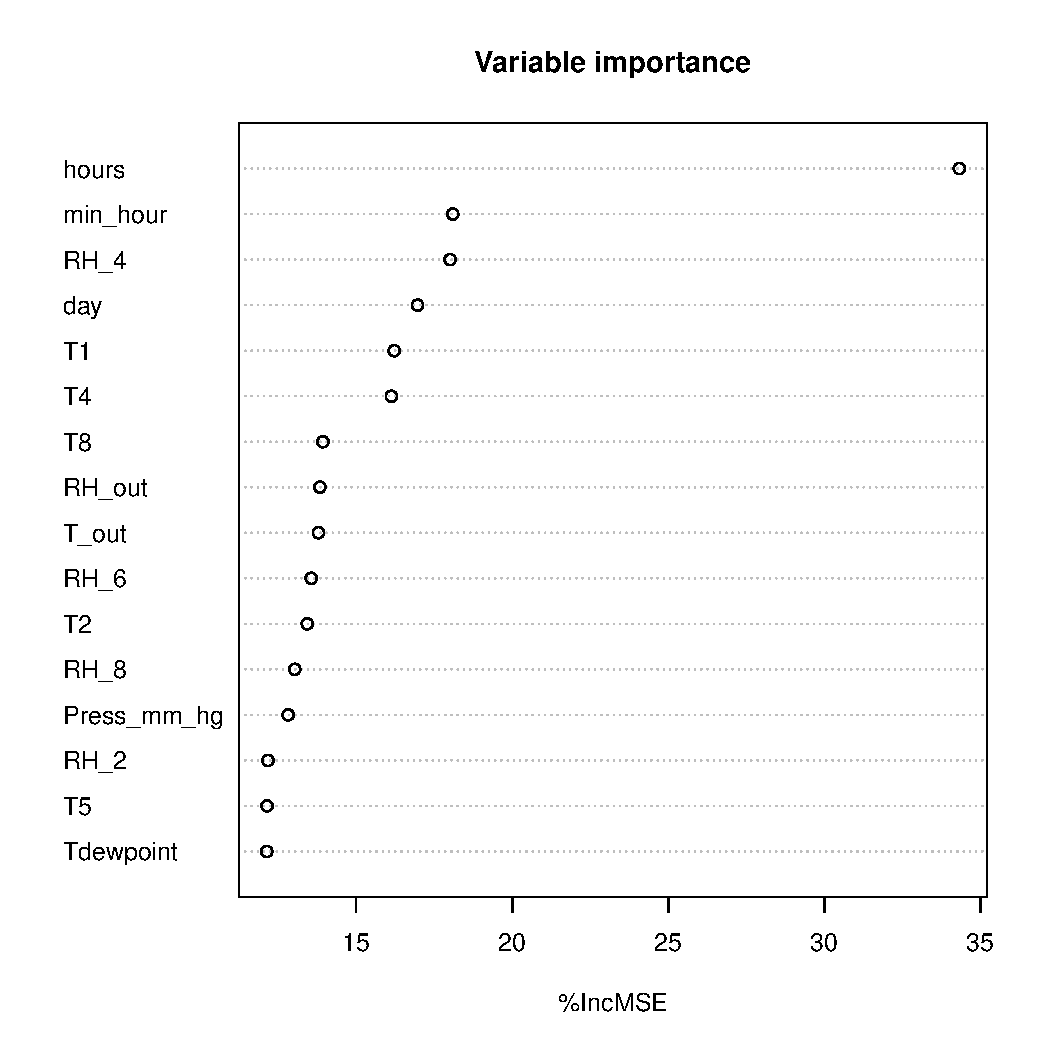
\includegraphics[page=1,
				width=0.8\linewidth,
				origin=c	
		]{../Rplots.pdf}
    }}%
    %\caption{TODO caption}%
    \label{FIG_1}%
\end{figure}

\endgroup



\begingroup
\let\clearpage\relax
\chapter{Selekcja atrybutów}

TODO jakoś ładnie opisać, to co niżej raczej dla inspiracji\\

%TODO zajebane z elka.mine
Algorytm randomForest pozwala uszeregować atrybuty na dwa sposoby:
\begin{itemize}
\item[$\bullet$] przydatność atrybutu oceniania jest względem tego, jak bardzo model pogorszy się gdy tego atrybutu zabraknie,
\item[$\bullet$] przydatność atrybutu określa zmniejszenie nieczystości po podziale w oparciu o ten atrybut.
\end{itemize}
Została wybrana pierwsza metoda ze względu na jej widoczny i bezpośredni związek z jakością całego modelu.

%TODO zajebane z twojego readme z gita
Najprostszym, zadowalającym rozwiązaniem jest zastosowanie pakietu randomForest w celu wyznaczenia predykcyjnej przydatności atrybutów, a następnie wybór (może w kilku wariantach) pewnej liczby najlepszych atrybutów (np. najlepsze 25\%, 50\% itp.). W tym przypadku zalecałbym użycie miary "mean decrease accuracy", co wymaga użycia w wywołaniu funkcji randomForest argumentu importance=TRUE, zaś w wywołaniu funkcji importance lub varImpPlot argumentu type=1. Inne bardziej zautomatyzowane podejścia można znaleźć w kilku pakietach wymienionych tutaj: {\url{https://github.com/FrancisArgnR/R-FeatureSelection-Packages}}

\section{Wyniki selekcji atrybutów}
TODO jakaś tabelka albo co + ew wnioski\\

\endgroup



\begingroup
\let\clearpage\relax
\chapter{Konstrukcja i ocena modeli}

\section{Metody konstrukcji modeli}
Pojedyncze modele drzew regresji zazwyczaj cierpią z powodu wysokiej wariancji -- jedną z metod jej redukcji jest tzw. Bagging (\textbf{B}ootstrap \textbf{agg}regat\textbf{ing}). 
Metoda ta polega na łączeniu i uśrednianiu wielu modeli drzew, co  zmniejsza wariancję i redukuje zbytnie dopasowanie.
%TODO dokładniejszy opis działania bo wydaje się mało
%Create m bootstrap samples from the training data. Bootstrapped samples allow us to create many slightly different data sets but with the same distribution as the overall training set.
%For each bootstrap sample train a single, unpruned regression tree.
%Average individual predictions from each tree to create an overall average predicted value.

Bagging może zostać zrealizowany za pomocą pakietu
\textit{ipred} 
lub
\textit{caret}. 
\textit{Ipred} jest z reguły prostszy w realizacji, jednakże stosowanie \textit{caret} niesie za sobą kilka zalet.
Znacznie prościej jest weryfikować krzyżowo wyniki -- pomimo możliwości wykorzystania błędu OOB (Out-of-Bag) w \textit{ipred}, weryfikacja krzyżowa daje dużo lepsze zrozumienie spodziewanego błędu. 
Dodatkowo możliwy jest dostęp do zmiennej odpowiedniości w wygenerowanych drzewach.
%TODO tłumaczenie potwierdź pls: We can assess variable importance across the bagged trees

%TODO który w końcu wybraliśmy
%TODO to co jest niżej jest zajebane z elka.mine, trzeba zmienić
Do konstrukcji modeli klasyfikacji został wykorzystany pakiet rpart budujacy drzewo klasyfikacji oraz pakiet
e1071, który umozliwia waidacje skrosna oraz automatyczny dobór parametrów w celu zmninimalizowania
błedu.

\section{Budowa modelu klasyfikacji z pakietu ipred}
%TODO pakiety R i parametry ~notatka z poprzedniego sprawka
TODO - pakiety R, parametry (np kryteria stopu, etc)

\section{Ocena modeli}
TODO opisać że wybraliśmy np: \\
CC - współczynnik korelacji liniowej Pearsona\\
\begin{gather*}
	\frac{cov(P,A)}{var(P) \cdot var(A)}
\end{gather*}

TODO tutaj ładnie się wpasuje co po kolei w kodzie poszło

\endgroup




\begingroup
\let\clearpage\relax
\chapter{Wnioski}

TODO\\

\endgroup


%%%%%%%%%%%%%%%%%%%%%%%%%%%%%%%%%%%%%%%%%%%%%%%%%%%%%%%%%%%%%   
% 		Załączniki z kodem
%%%%%%%%%%%%%%%%%%%%%%%%%%%%%%%%%%%%%%%%%%%%%%%%%%%%%%%%%%%%%

%TODO nie wiem czy to potrzebne, ale daje objętość

\lstset{language=R, 
		basicstyle=\ttfamily\small,
		frame=lines,
		numbers=left,
		numberstyle=\small\color{blue},
		showtabs=true}
		
\pagebreak
Plik: main.r
\lstinputlisting{../R/main.r}
\clearpage

\pagebreak
Plik: data{\_}org.R
\lstinputlisting{../R/data_org.R}
\clearpage

\pagebreak
Plik: feature{\_}selection.R
\lstinputlisting{../R/feature_selection.R}
\clearpage

\pagebreak
Plik: simple.filter.R
\lstinputlisting{../R/simple.filter.R}
\clearpage

\pagebreak
Plik: model{\_}eval.R
\lstinputlisting{../R/model_eval.R}
\clearpage

\end{document}
